\documentclass{beamer}
\usepackage[utf8]{inputenc}

\usetheme{Madrid}
\usecolortheme{default}
\usepackage{amsmath,amssymb,amsfonts,amsthm}
\usepackage{txfonts}
\usepackage{multicol}
\usepackage{tkz-euclide}
\usepackage{listings}
\usepackage{adjustbox}
\usepackage{array}
\usepackage{tabularx}
\usepackage{gvv}
\usepackage{lmodern}
\usepackage{circuitikz}
\usepackage{tikz}
\usepackage{graphicx}

\setbeamertemplate{page number in head/foot}[totalframenumber]

\usepackage{tcolorbox}
\tcbuselibrary{minted,breakable,xparse,skins}



\definecolor{bg}{gray}{0.95}
\DeclareTCBListing{mintedbox}{O{}m!O{}}{%
  breakable=true,
  listing engine=minted,
  listing only,
  minted language=#2,
  minted style=default,
  minted options={%
    linenos,
    gobble=0,
    breaklines=true,
    breakafter=,,
    fontsize=\small,
    numbersep=8pt,
    #1},
  boxsep=0pt,
  left skip=0pt,
  right skip=0pt,
  left=25pt,
  right=0pt,
  top=3pt,
  bottom=3pt,
  arc=5pt,
  leftrule=0pt,
  rightrule=0pt,
  bottomrule=2pt,
  toprule=2pt,
  colback=bg,
  colframe=orange!70,
  enhanced,
  overlay={%
    \begin{tcbclipinterior}
    \fill[orange!20!white] (frame.south west) rectangle ([xshift=20pt]frame.north west);
    \end{tcbclipinterior}},
  #3,
}
\lstset{
    language=C,
    basicstyle=\ttfamily\small,
    keywordstyle=\color{blue},
    stringstyle=\color{orange},
    commentstyle=\color{green!60!black},
    numbers=left,
    numberstyle=\tiny\color{gray},
    breaklines=true,
    showstringspaces=false,
}
%------------------------------------------------------------
%This block of code defines the information to appear in the
%Title page
\title %optional
{2.10.33}
\date{September 8,2025}
%\subtitle{A short story}

\author % (optional)
{Aditya Appana - EE25BTECH11004}



\begin{document}


\frame{\titlepage}
\begin{frame}{Question}
Let $\alpha , \beta, \gamma$ be distinct real numbers. The points with position vectors $\alpha\hat{i} + \beta\hat{j} + \gamma\hat{k}$, $\beta\hat{i} +\gamma\hat{j} + \alpha\hat{k}$, $\gamma\hat{i} + \alpha\hat{j} + \beta\hat{k}$:

\begin{enumerate}\begin{multicols}{2}
    \item are collinear
    \item form an equilateral triangle
    \item form a scalene triangle
    \item form a right angled triangle
    \end{multicols}
\end{enumerate}
\end{frame}



\begin{frame}[fragile]
    \frametitle{Solution}

To answer this question, we need to find the distance between each of these points.

Let $\vec{A}$ be \myvec{\alpha \\ \beta \\ \gamma}, $\vec{B}$ be \myvec{ \beta \\ \gamma \\ \alpha}, and $\vec{C}$ be \myvec{\gamma \\ \alpha \\ \beta}. \\

First, we need to check when the three points are collinear. We can do this using the collinearity matrix: \begin{align}\myvec{\vec{C}-\vec{A} & \vec{B} - \vec{A}}^T\end{align}If the rank of the matrix is 1, then the points are collinear.

    
\begin{align}
\myvec{\gamma - \alpha & \alpha - \beta & \beta - \gamma \\ \beta - \alpha & \gamma - \beta & \alpha - \gamma}
\end{align}


\end{frame}


\begin{frame}[fragile]
    \frametitle{Solution}
    
The rank of this matrix will be 1 only when all the elements in the bottom row of the matrix are equal to 0. This occurs only when $\alpha = \beta = \gamma$, which contradicts the fact that $\alpha, \beta, \gamma$ are distinct.\\

Therefore the points must be non-collinear and form a triangle.\\

The sides of the triangle are $\vec{A} - \vec{B}, \vec{B} - \vec{C}, \vec{C}- \vec{A}$.\\

\end{frame}


\begin{frame}[fragile]
    \frametitle{Solution}
\begin{align}
\vec{A-B} = \myvec{\alpha - \beta \\ \beta - \gamma \\ \gamma - \alpha} \\
\vec{B-C} = \myvec{\beta - \gamma \\ \gamma - \alpha \\ \alpha - \beta} \\
\vec{C-A} = \myvec{\gamma - \alpha \\ \alpha - \beta \\ \beta - \gamma}
\end{align}


$\norm{\vec{A}-\vec{B}} = \norm{\vec{B}-\vec{C}} = \norm{\vec{C}-\vec{A}} = \sqrt{(\alpha - \beta)^2  + (\beta - \gamma)^2 + (\gamma - \alpha)^2}$ 


The three points therefore form an \textbf{equilateral triangle}, so option (2) is correct.

\end{frame}


\begin{frame}[fragile]
\frametitle{Python Code}
\begin{lstlisting}
import numpy as np


vector = np.zeros(3)
vector[0] = input()
vector[1] = input()
vector[2] = input()

print(np.linalg.norm(vector))

A = np.array([vector[0],vector[1],vector[2]])
B = np.array([vector[1],vector[2],vector[0]])
C = np.array([vector[2],vector[0],vector[1]])

fig = plt.figure(figsize = (6,6))
\end{lstlisting}
\end{frame}

\begin{frame}[fragile]
\frametitle{Python Code}
\begin{lstlisting}
ax = fig.add_subplot(111, projection='3d')

AB = line_gen(A,B)
BC= line_gen(B,C)
CA= line_gen(C,A)

plt.plot(AB[0,:],AB[1,:],AB[2,:],label='$AB$')
plt.plot(BC[0,:],BC[1,:],BC[2,:],label='$BC$')
plt.plot(CA[0,:],CA[1,:],CA[2,:],label='$CA$')

ax = plt.gca()
ax.spines['top'].set_color('none')
ax.spines['left'].set_position('zero')
ax.spines['right'].set_color('none')
ax.spines['bottom'].set_position('zero')

plt.grid()
plt.axis('equal')
plt.show()

\end{lstlisting}

\end{frame}


\begin{frame}[fragile]
\frametitle{C Code}
\begin{lstlisting}
#include<stdio.h>
#include<math.h>

float norm(float a, float b, float c){

float answer;
answer = pow(a,2) + pow(b,2) + pow(c,2);
answer = sqrt(answer);

return answer;

}
\end{lstlisting}
\end{frame}


\begin{frame}[fragile]
\frametitle{Python and C Code}
\begin{lstlisting}
import numpy as np
import ctypes
c_lib=ctypes.CDLL('./5c.so')

c_lib.norm.argtypes = [ctypes.c_float, ctypes.c_float, ctypes.c_float]
c_lib.norm.restype = ctypes.c_float

vector = np.zeros(3)
vector[0] = input()
vector[1] = input()
vector[2] = input()

answer = c_lib.norm(
    ctypes.c_float(vector[0]),
    ctypes.c_float(vector[1]), 
    ctypes.c_float(vector[2]))
print(answer)

A = np.array([vector[0],vector[1],vector[2]])
B = np.array([vector[1],vector[2],vector[0]])
C = np.array([vector[2],vector[0],vector[1]])

fig = plt.figure(figsize = (6,6))

\end{lstlisting}
\end{frame}

\begin{frame}[fragile]
\frametitle{Python and C Code}
\begin{lstlisting}
ax = fig.add_subplot(111, projection='3d')

AB = line_gen(A,B)
BC= line_gen(B,C)
CA= line_gen(C,A)

plt.plot(AB[0,:],AB[1,:],AB[2,:],label='$AB$')
plt.plot(BC[0,:],BC[1,:],BC[2,:],label='$BC$')
plt.plot(CA[0,:],CA[1,:],CA[2,:],label='$CA$')

ax = plt.gca()
ax.spines['top'].set_color('none')
ax.spines['left'].set_position('zero')
ax.spines['right'].set_color('none')
ax.spines['bottom'].set_position('zero')

plt.grid()
plt.axis('equal')
plt.show()

\end{lstlisting}
\end{frame}

\begin{frame}[fragile]
\frametitle{Plot}

For example, let us take $\alpha = 2$, $\beta = 1$, $\gamma = 3$.
We get an equilateral triangle as shown below:

\begin{figure}[H]
    \centering
    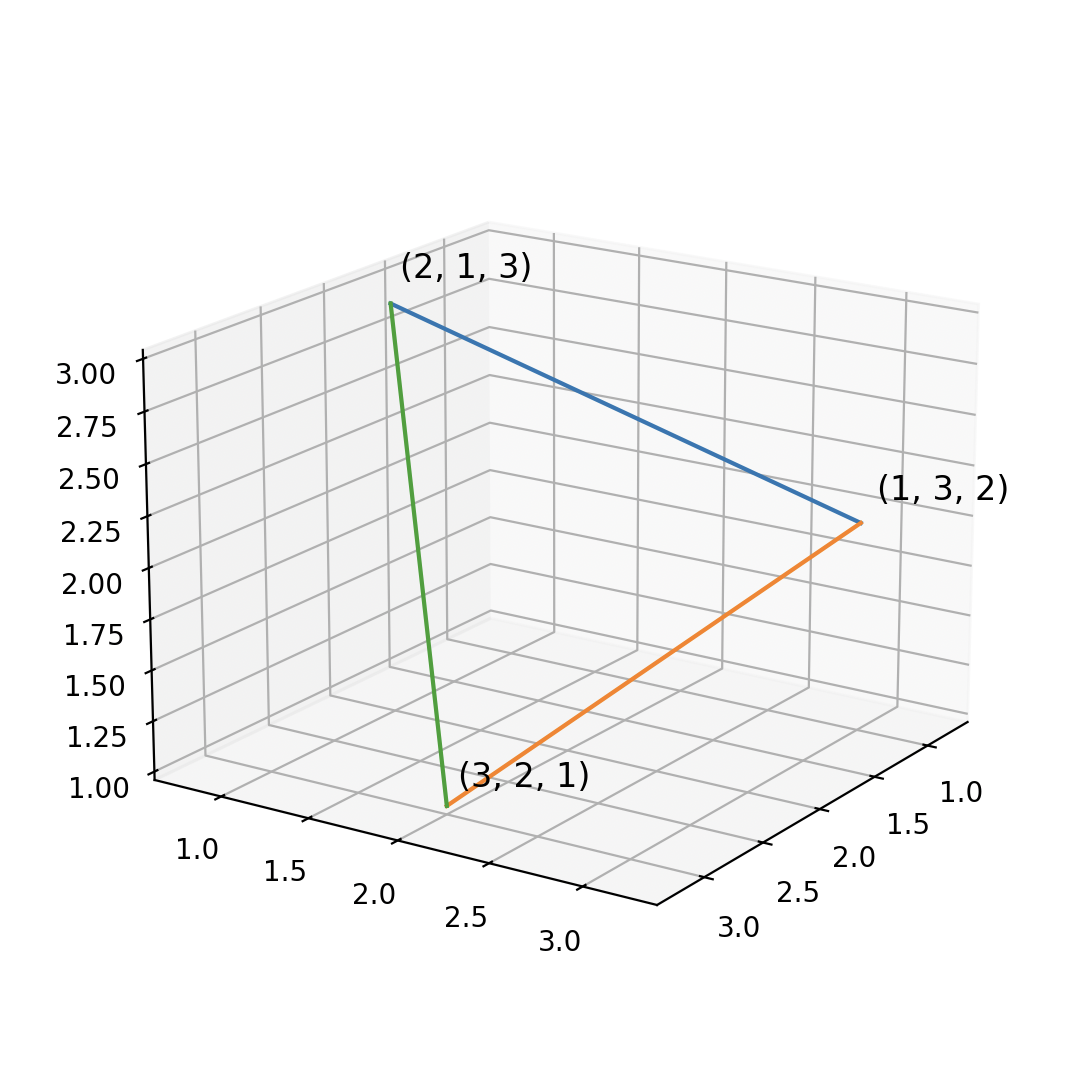
\includegraphics[width=0.6\columnwidth]{Figs/Example.png}
    \caption{Equilateral Triangle}
    \label{fig:placeholder}
\end{figure}

\end{frame}

\end{document}